% !TEX root = ../main.tex
% chktex-file 21
% chktex-file 46
\section{Effects of Coarsening}%
\label{sec:cons}

We have just seen how to compute a coarsened graph $G_c$ via the REC algorithm.
What remains to be answered now is how coarsening affects the performance of graph algorithms when $G_c$ is used as a proxy for the original graph $G$.
In the first step we will introduce a graph similarity measure.
Using this measure we will then put bounds on the dissimilarity of $G$ and $G_c$.
Finally we will use those bounds to analyze the influence of coarsening on the performance of the \textit{spectral clustering algorithm}.

\subsection{Restricted Spectral Similarity}%
\label{sec:cons:rss}

To compare a graph $G$ with its coarsened version $G_c$ we will use the notion of \textit{spectral similarity}.
As we have seen before, $G$ can be viewed as an operator that transforms an input signal $x \in \mathbb{R}^N$.
We described this transform in terms of the graph's Laplacian $L$,
more specifically in terms of the Laplacian's eigenbasis ${\{ u_k \}}_{1 \leq k \leq N}$ and spectrum ${\{ \lambda_k \}}_{1 \leq k \leq N}$.
Similarly the coarsened graph $G_c$ can be described in terms of its Laplacian $L_c$.
Since $L \in \mathbb{R}^{N \times N}$ and $L_c \in \mathbb{R}^{n \times n}$ act on signal spaces of different dimensionality, they cannot be compared directly however.
Instead we compare $L$ with $\widetilde{L} = C^{\top} L_c C$, the upsampled version of $L_c$.
We say $\widetilde{L}$ is an \textit{$\epsilon$-approximation} of $L$ iff.\  $\widetilde{L}$ scales the eigenvectors $u_k$ of $L$ by a factor of roughly $\lambda_k$ in the direction of $u_k$:
\begin{wrapfigure}{r}{0.25\textwidth}
	\centering
	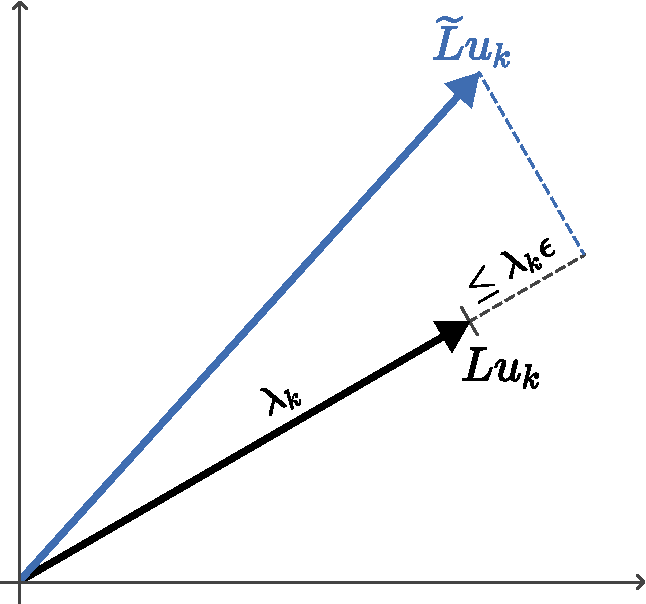
\includegraphics[width=\linewidth]{gfx/cons/rss.pdf}
	\caption{See \cref{eq:cons:rss}.}\label{fig:cons:rss}
\end{wrapfigure}
\begin{align}
	\forall k \leq K:\ (1 - \epsilon) \underbrace{u_k^{\top} L u_k}_{\lambda_k} \leq u_k^{\top} \widetilde{L} u_k \leq (1 + \epsilon) \underbrace{u_k^{\top} L u_k}_{\lambda_k} \text{ with } \epsilon \geq 0\label{eq:cons:rss}
\end{align}
The reason we require \cref{eq:cons:rss} to hold only for the first $K$ eigenvectors of $L$ is, that $\text{rank}(L) = N - c$, whereas $\text{rank}(\widetilde{L}) = n - c$;
i.e.\ $\widetilde{L}$ has a higher dimensional null space\footnote{%
	Here $c$ denotes the number of connected components of $G$.
	They reduce the rank since $\lambda_1 = \cdots = \lambda_c = 0$.
}.
Thus \cref{eq:cons:rss} cannot not hold for a signal $x$ that is in the null space of $\widetilde{L}$ but not in that of $L$.
For this reason the similarity condition is restricted to the first $K$ eigenvectors, as they represent the most important ``low-frequency'' components of $G$.
This restricted condition is called \textit{restricted spectral similarity} (RSS).

The choice of $K$ in RSS depends on the level of detail that should be considered when comparing $L$ and $\widetilde{L}$.
If $G$ has $c'$ clusters, i.e.\ connected subgraphs with relatively few edges going out of it, a choice of $K = c'$ is typically reasonable.
That way RSS checks whether the clusters of $G$ are preserved in the coarsened graph $G_c$ and how much the connectedness between the clusters changes.
Details like the connections within clusters on the other hand would not have a strong influence on the RSS similarity.

\subsection{Putting an RSS-bound on REC}%
\label{sec:cons:bound}

\subsection{Implications for Spectral Clustering}%
\label{sec:cons:sc}
